\documentclass[a4paper,12pt]{article}

\setlength{\textwidth}{15.0cm}
\setlength{\textheight}{24.0cm}
\setlength{\topmargin}{0cm}
\setlength{\headsep}{0cm}
\setlength{\headheight}{0cm}
\pagestyle{plain}

\usepackage{hyperref}
\hypersetup{
    colorlinks=true,
    linkcolor=blue,
    filecolor=magenta,      
    urlcolor=blue,
    citecolor=blue,
    linktoc=page
}
\usepackage[dvips]{epsfig}
\usepackage{tikz}
\usepackage[english]{babel}
\usepackage{caption}
\captionsetup{font=it}
\usepackage[autostyle, english=american]{csquotes}

\usepackage[
backend=biber,
style=alphabetic,
]{biblatex}

\renewcommand{\bibfont}{\footnotesize}

\usepackage{amsmath,amssymb,amsthm}

\usepackage{comment}
\usepackage{listings}

% \addbibresource{bibliography2.bib} 
\setlength{\parindent}{0pt}

\selectlanguage{english}
\begin{document}

\title{Project 2023-2024: Simulation of the Double Slit Experiment
    and simulation of Wi-Fi signals at home}
\author{Isidoor Pinillo Esquivel}
\date{\today}
\maketitle


\section{Implementation of Exterior Complex Scaling (ECS) Boundary Conditions}
\subsection{Equivalence Between Complex Grid and Complex Wave Number}

The homogenous discretized Helmholtz equation ECS is equivalent to
to the Helmholtz equation with a complex wave number.
Let $h$ be the normal "real" grid spacing and $\tilde{h} = z h, z \in \mathbb{C} $
be the complex grid spacing.
Let $\sigma$ be the normal real wave number and $\tilde{\sigma} = z^{2} \sigma$ be the complex wave number.
Let $u$ be the solution to the discretized Helmholtz equation with a complex wave number on a normal grid
and $\tilde{u}$ be the solution to the discretized Helmholtz equation on the complex grid.

\begin{align}
    \frac{\tilde{u}(\tilde{x}-\tilde{h}) -2 \tilde{u}(\tilde{x}) + \tilde{u}(\tilde{x} - \tilde{h})}{\tilde{h}^2} + \sigma \tilde{u} & = 0  \Leftrightarrow \\
    \frac{\tilde{u}(\tilde{x}-zh) -2 \tilde{u}(\tilde{x}) + \tilde{u}(\tilde{x} - zh)}{z^{2}h^2} + \sigma \tilde{u}                  & = 0  \Leftrightarrow \\
    \frac{u(x-h) -2 u(x) + u(x - h)}{h^2} + z^{2} \sigma u                                                                           & = 0  \Leftrightarrow \\
    \frac{u(x-h) -2 u(x) + u(x - h)}{h^2} + \tilde{\sigma} u                                                                         & = 0
\end{align}

This equivalence does not hold when there is a source term.

\subsection{Non-Uniform Helmholtz Matrix Implementation}
Our implementation of the non-uniform of the Helmholtz equation uses following discretization scheme:
$$
    (\Delta_{h}u)_{i} = -\left( \frac{u_{i+1} - u_{i}}{h_{i+1/2}} - \frac{u_{i} - u_{i-1}}{h_{i-1/2}} \right) \frac{2}{h_{i+1/2} +h_{i-1/2}}
    .
$$

\subsection{Interpolation Matrix Construction}

The interpolation matrix is based on linear interpolation on a irregular grid, we only use
the real part of the complex grid to do interpolation. The restriction operation is defined
through the variational property.

\subsection{Validation of V-cycle Implementation with Test Problem}

We test our implementation of the V-cycle on a point source problem with $\sigma = -10$.

\begin{figure}[h!]
    \centering
    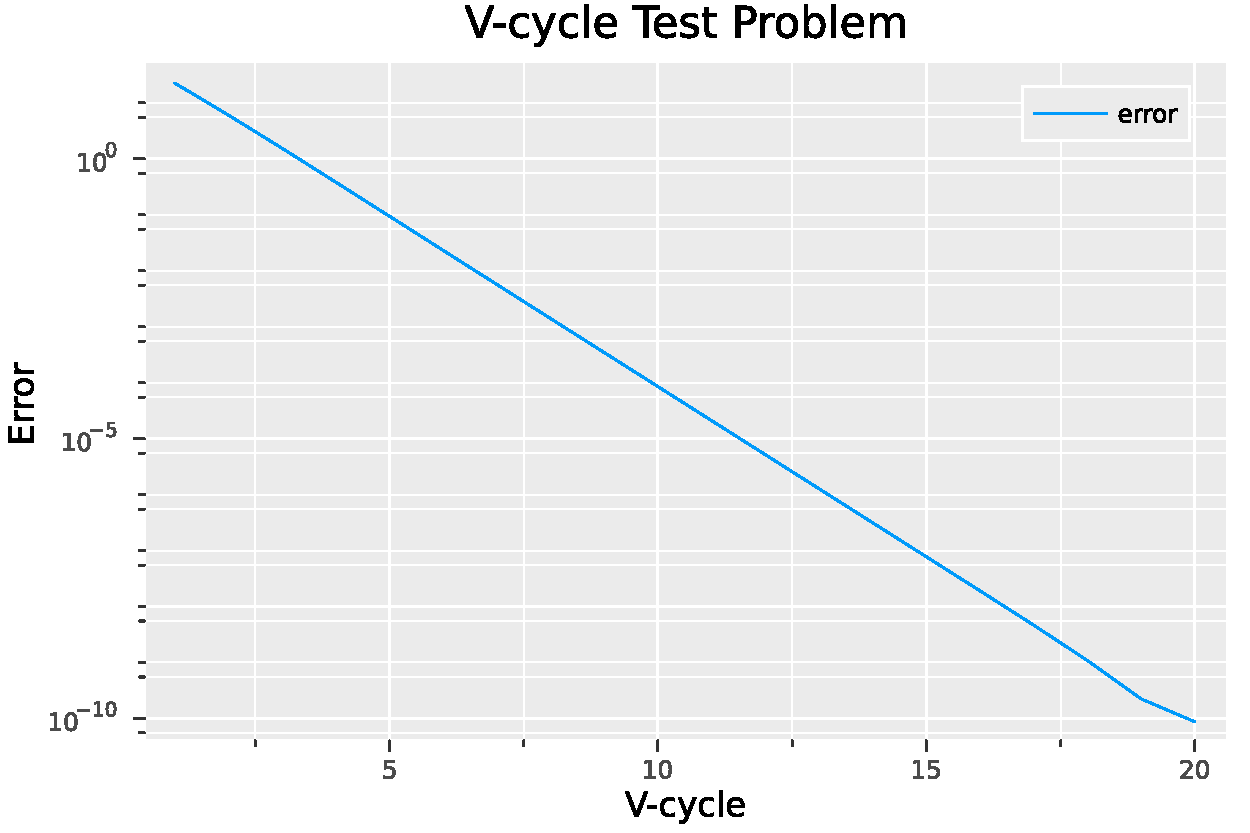
\includegraphics[width=0.8\textwidth]{../plots/Vcycle_Test_Problem.pdf}
    \caption{Convergence of the V-cycle for the test problem, demonstrating that the algorithm has been implemented correctly.}
    \label{fig:../plots/Vcycle_Test_Problem.pdf}
\end{figure}

\begin{figure}[h!]
    \centering
    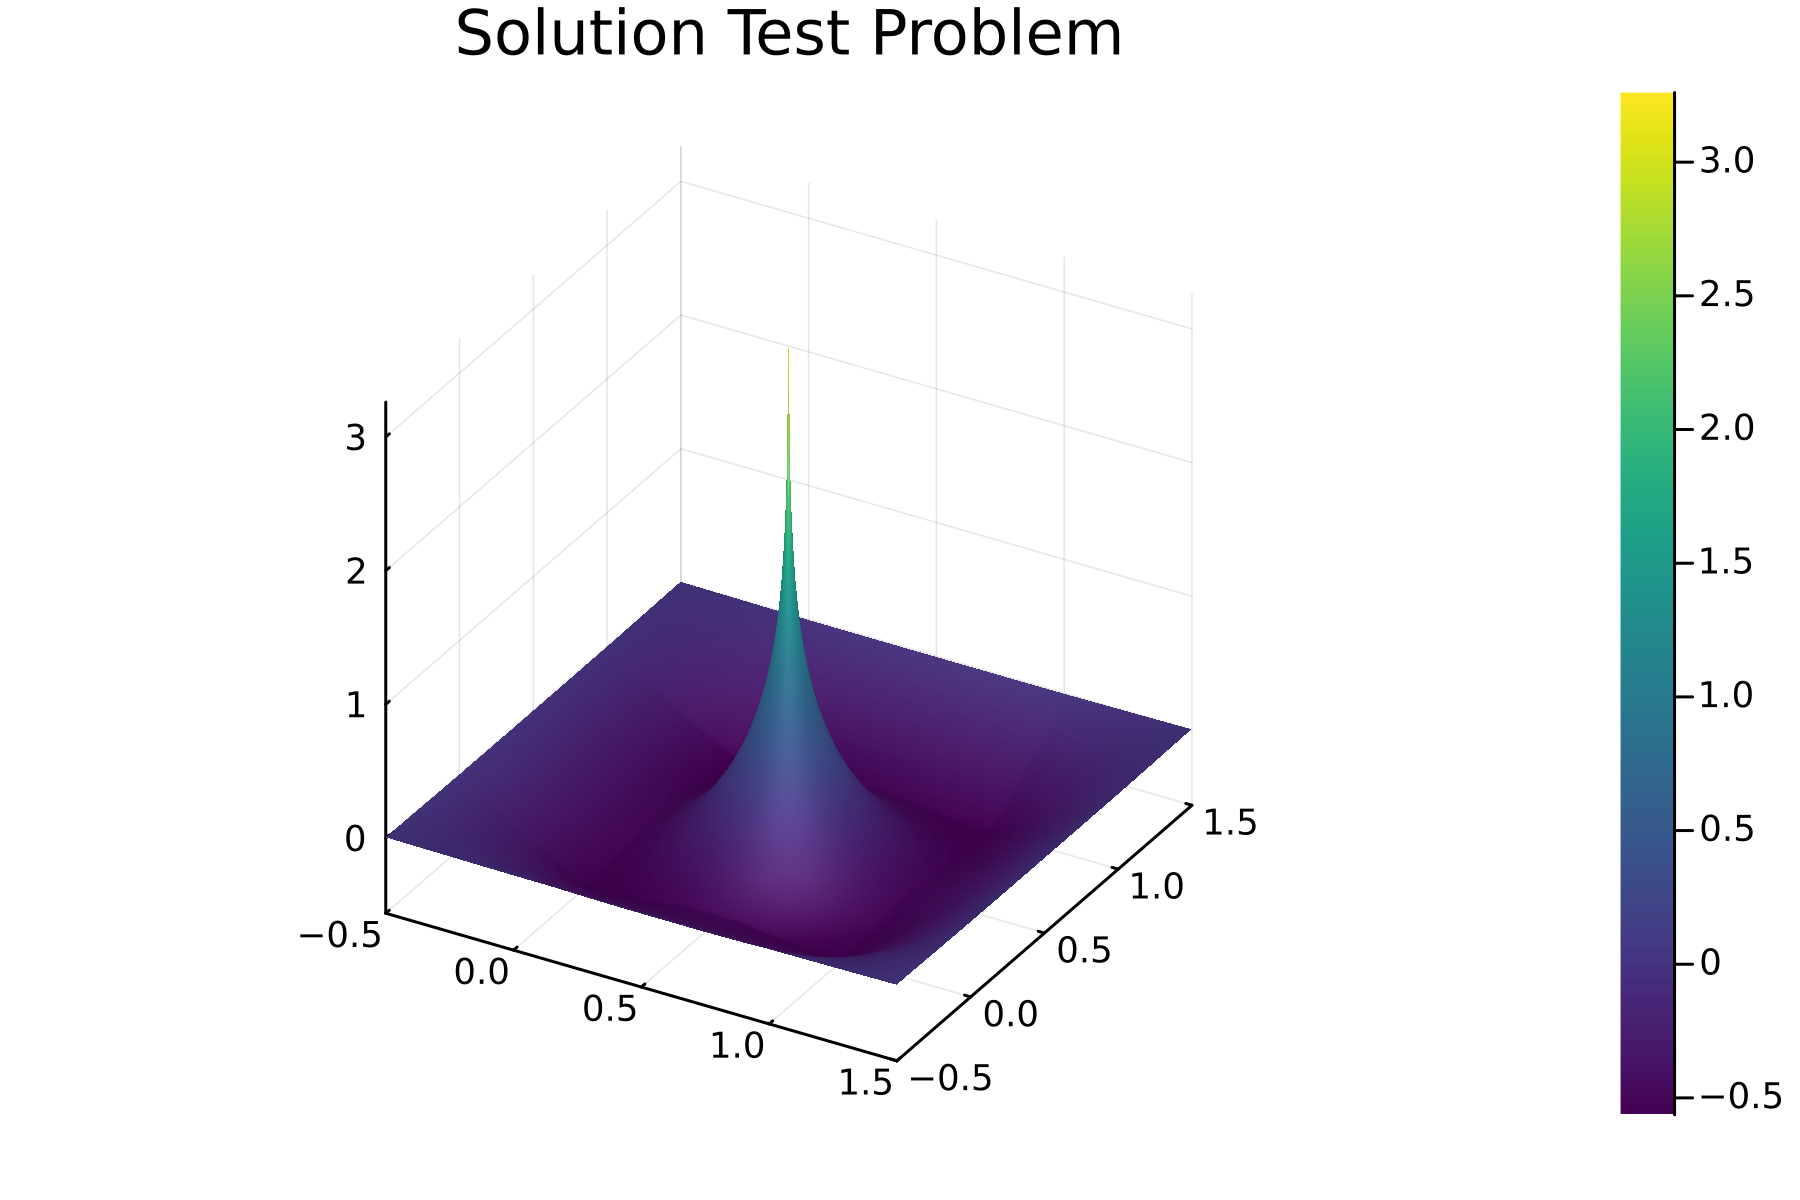
\includegraphics[width=0.8\textwidth]{../plots/Solution_Test_Problem.pdf}
    \caption{Computed solution for the test problem.}
    \label{fig:Solution_Test_Problem}
\end{figure}

\section{Simulation of Double Slit Experiment}
\subsection{Normal Wavenumber}

In our previous project, we examined the divergence of the Helmholtz equation with a homogeneous wavenumber.
It is not unexpected that introducing inhomogeneity to the wavenumber does not alter the divergence behavior
of the multigrid method.

\begin{figure}[h!]
    \centering
    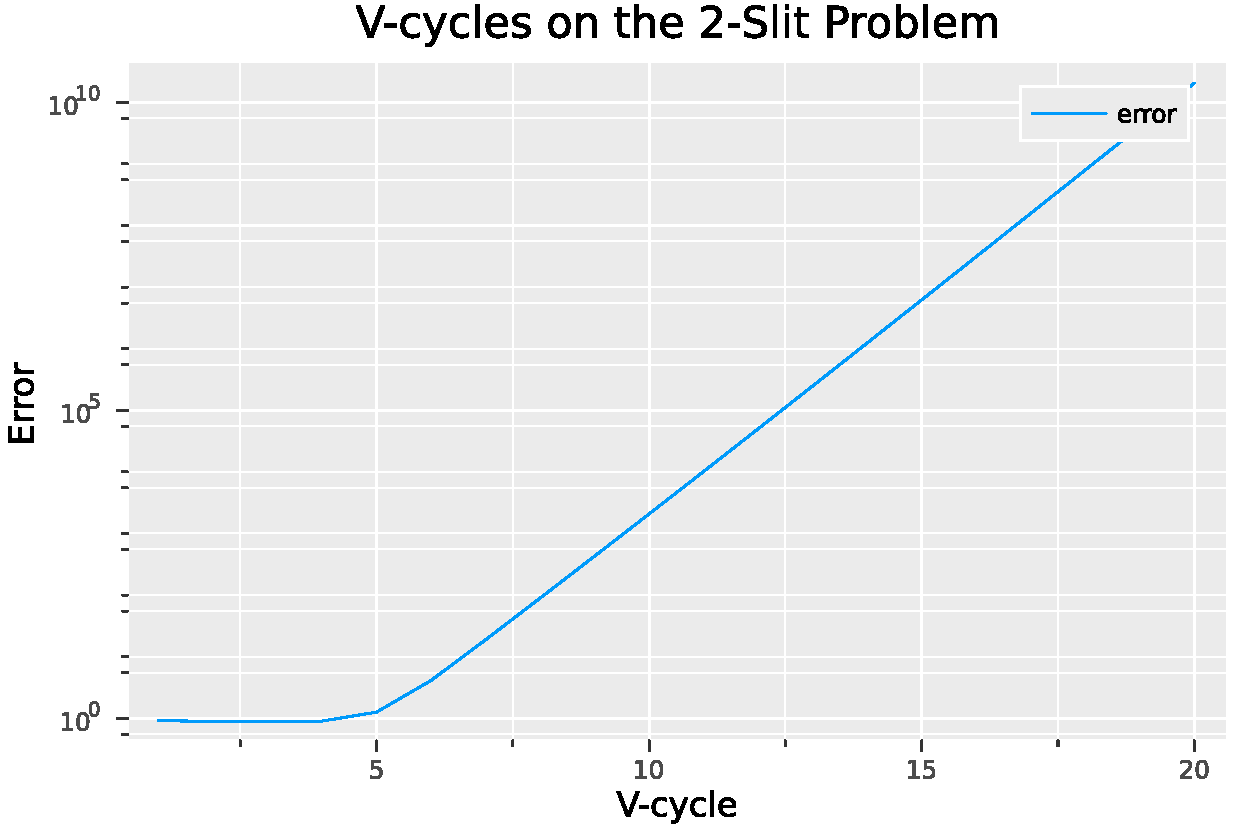
\includegraphics[width=0.8\textwidth]{../plots/Convergence_of_V-cycles_on_the_2-Slit_Problem.pdf}
    \caption{Divergence of V-cycles on the 2-Slit Problem.}
    \label{fig:Convergence_of_V-cycles_on_the_2-Slit_Problem}
\end{figure}

\subsection{Spectral Analysis of ECS Poisson Operator}
Adding ECS to the Poisson operator makes some eigenvalues complex, but this does not explain the
divergent behavior of multigrid. The divergence can be explained by the spectral properties of the Helmholtz
operator.

\subsection{Shifted Wavenumber}
Similar to Project 1, adding a complex shift makes multigrid converge.
\begin{figure}[h!]
    \centering
    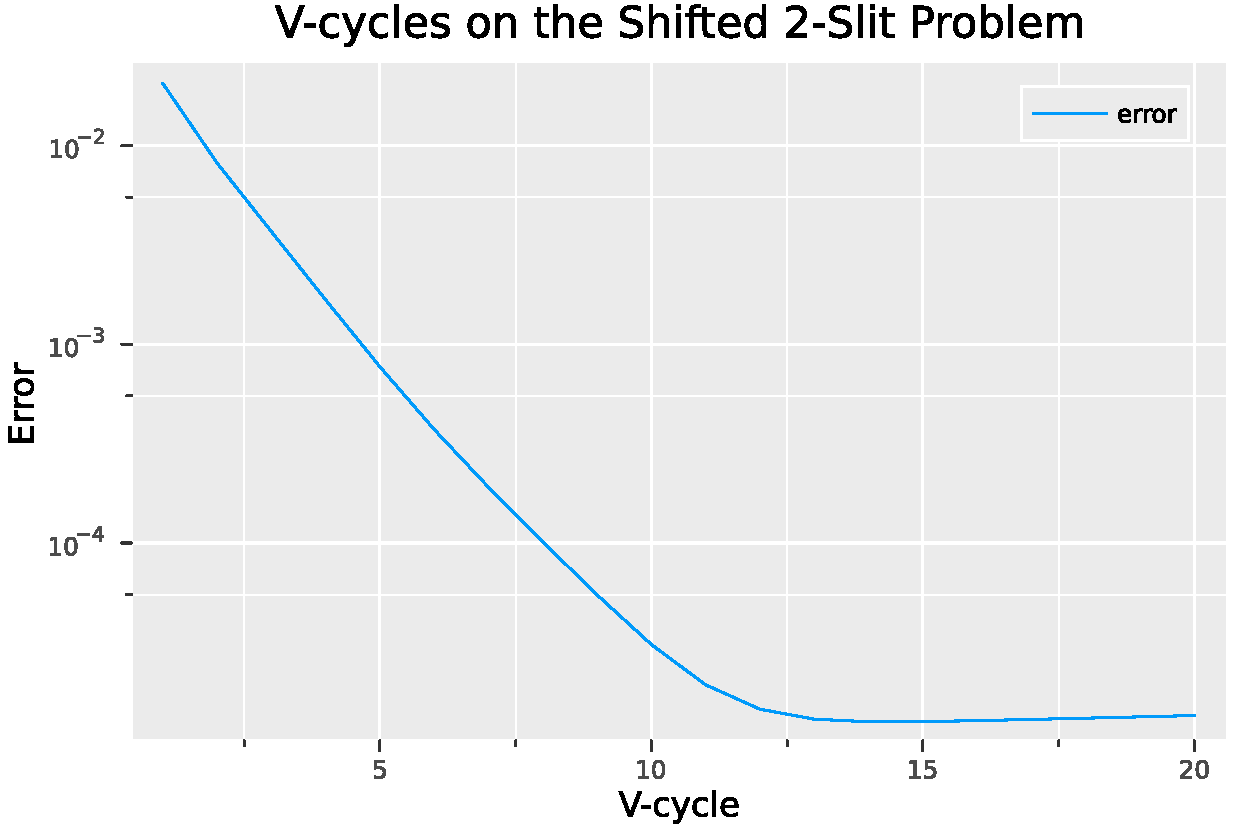
\includegraphics[width=0.8\textwidth]{../plots/Vcycles_shifted2slit.pdf}
    \caption{Convergence of V-cycles with shifted wavenumber.}
    \label{fig:../plots/Vcycles_shifted2slit.pdf}
\end{figure}

\subsection{Preconditioned GMRES}
The shifted problem can serve as a preconditioner for the non-shifted problem.
\begin{figure}[h!]
    \centering
    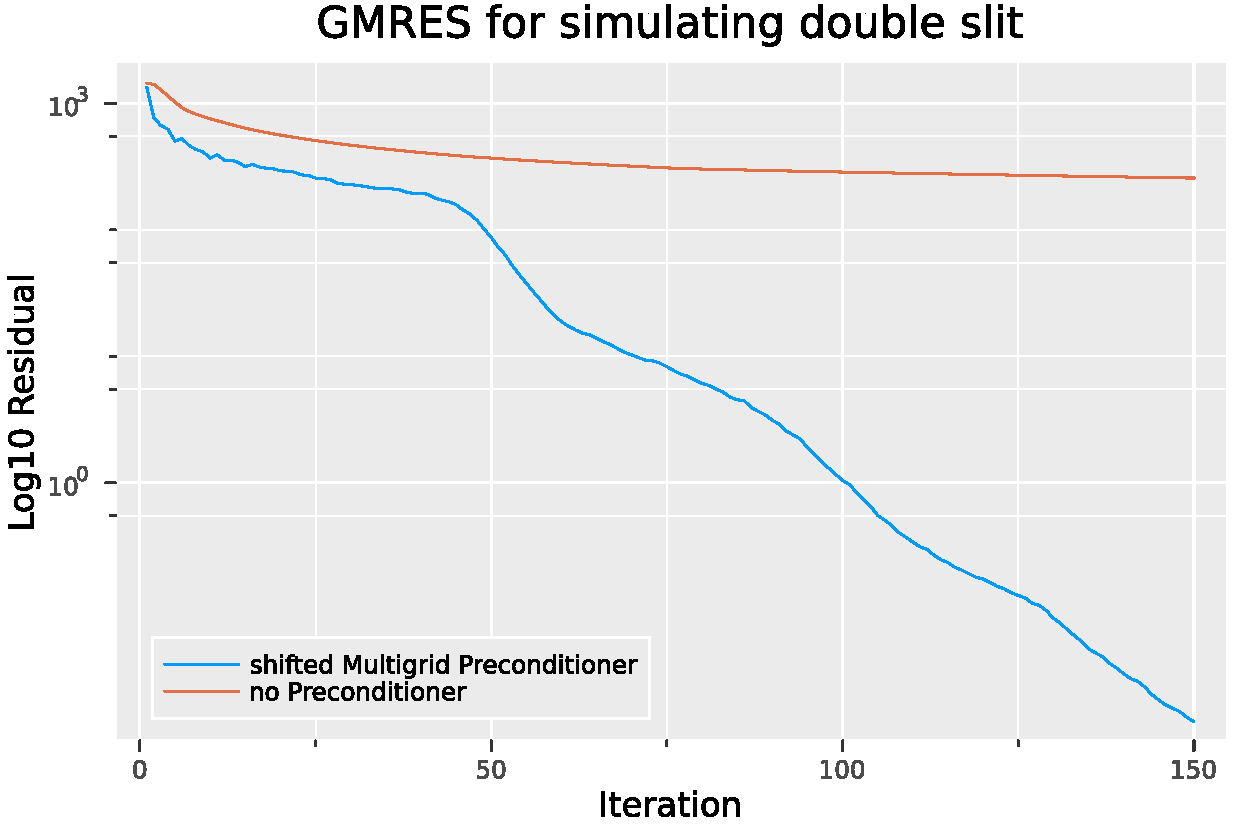
\includegraphics[width=0.8\textwidth]{../plots/GMRES2slit.pdf}
    \caption{Convergence of Preconditioned GMRES}
    \label{fig:../plots/GMRES2slit.pdf}
\end{figure}

\section{Simulation of Wi-Fi Signal Propagation at Home}

\subsection{Construction of Wavenumber and Source Representation}
We utilized GitHub Copilot to construct the wavenumber and the source, which represents the house.

\begin{figure}[h!]
    \centering
    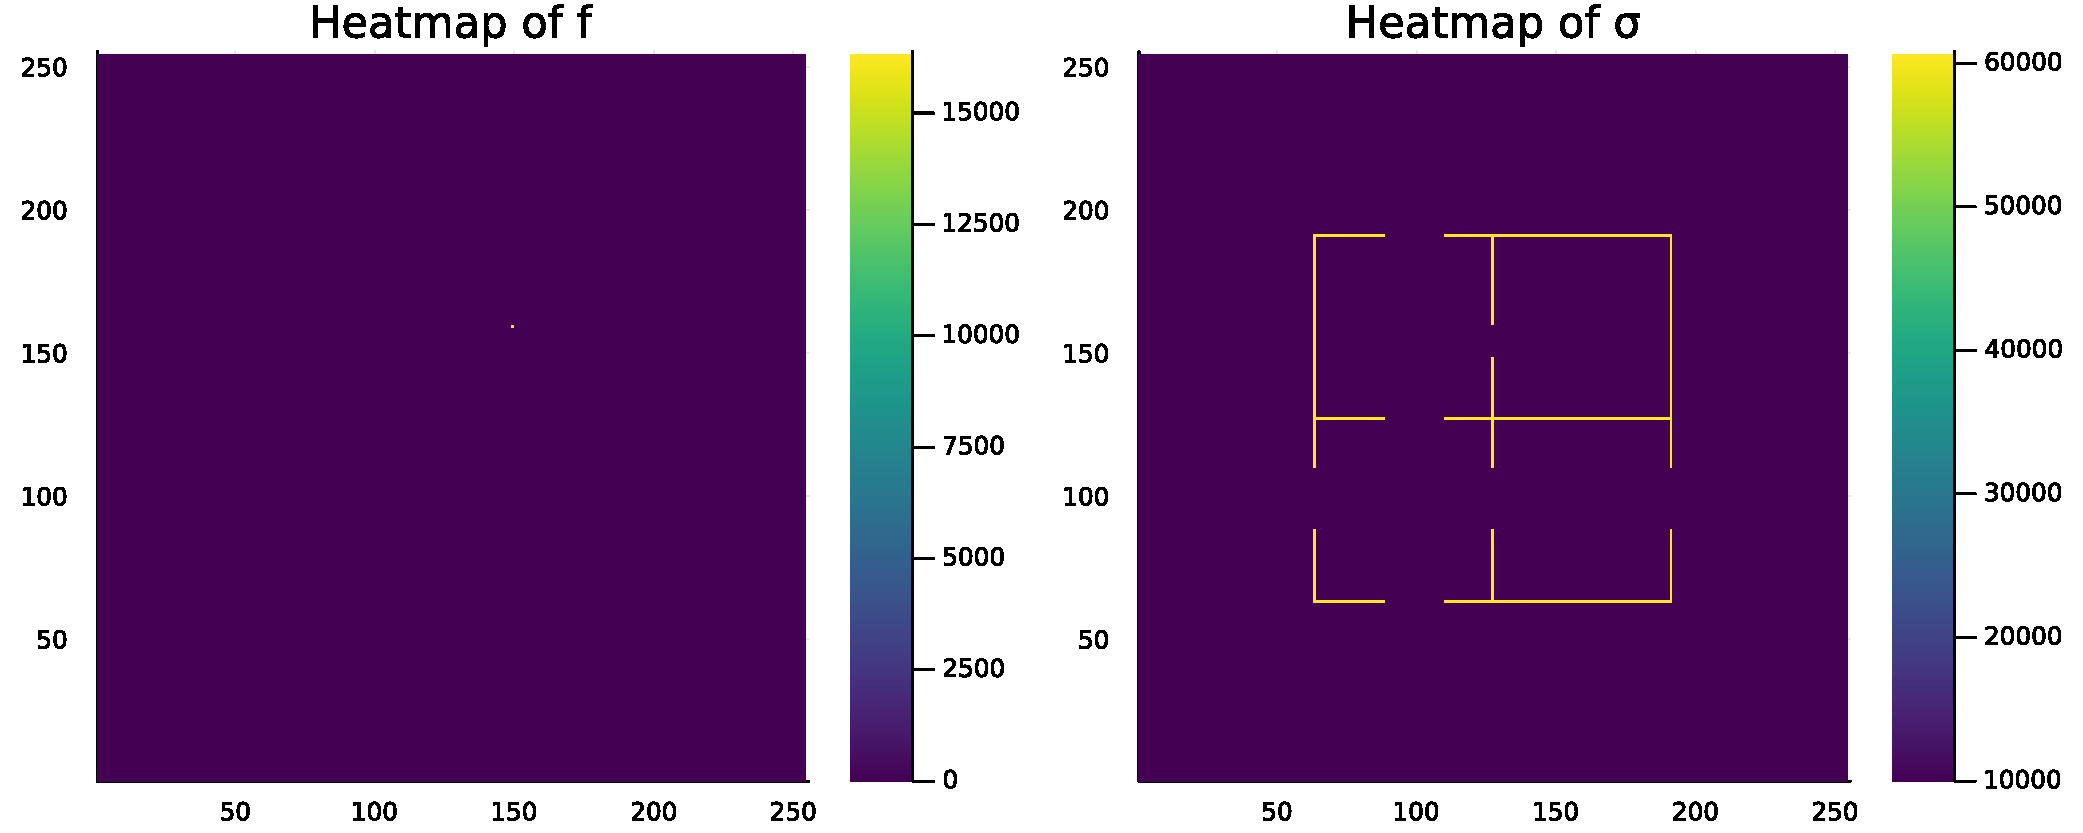
\includegraphics[width=0.8\textwidth]{../plots/wifi_setup.pdf}
    \caption{Setup for the Wi-Fi Signal Simulation Problem}
    \label{fig:../plots/wifi_setup.pdf}
\end{figure}

\subsection{Preconditioned GMRES for Wi-Fi Signal Simulation}

This is analogous to the 2-slit problem, where we use the shifted problem as a
preconditioner for the non-shifted problem. The convergence of GMRES takes
longer due to the more challenging behavior of the wavenumber.

\begin{figure}[h!]
    \centering
    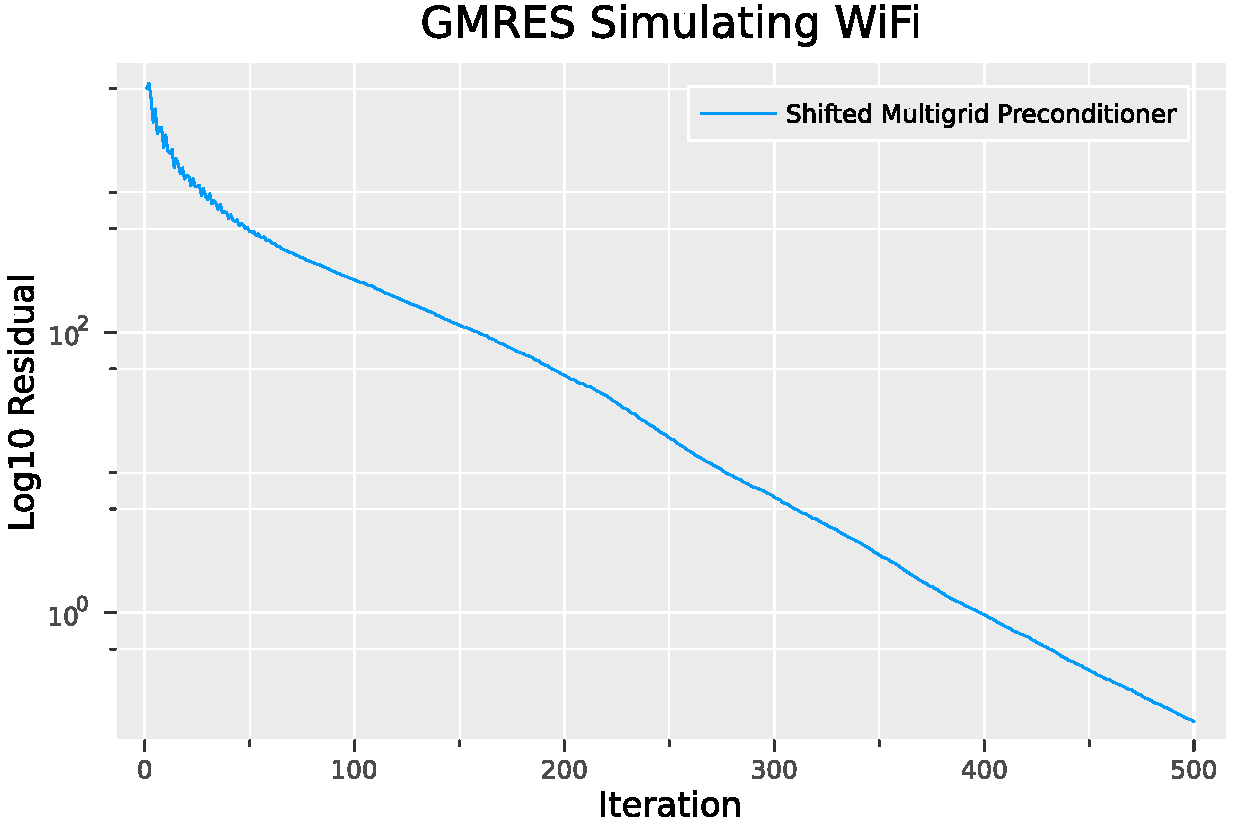
\includegraphics[width=0.8\textwidth]{../plots/gmres_wifi.pdf}
    \caption{Convergence of Preconditioned GMRES }
    \label{fig:../plots/gmres_wifi.pdf}
\end{figure}

Below, we present the computed solution to the Wi-Fi problem.

\begin{figure}[h!]
    \centering
    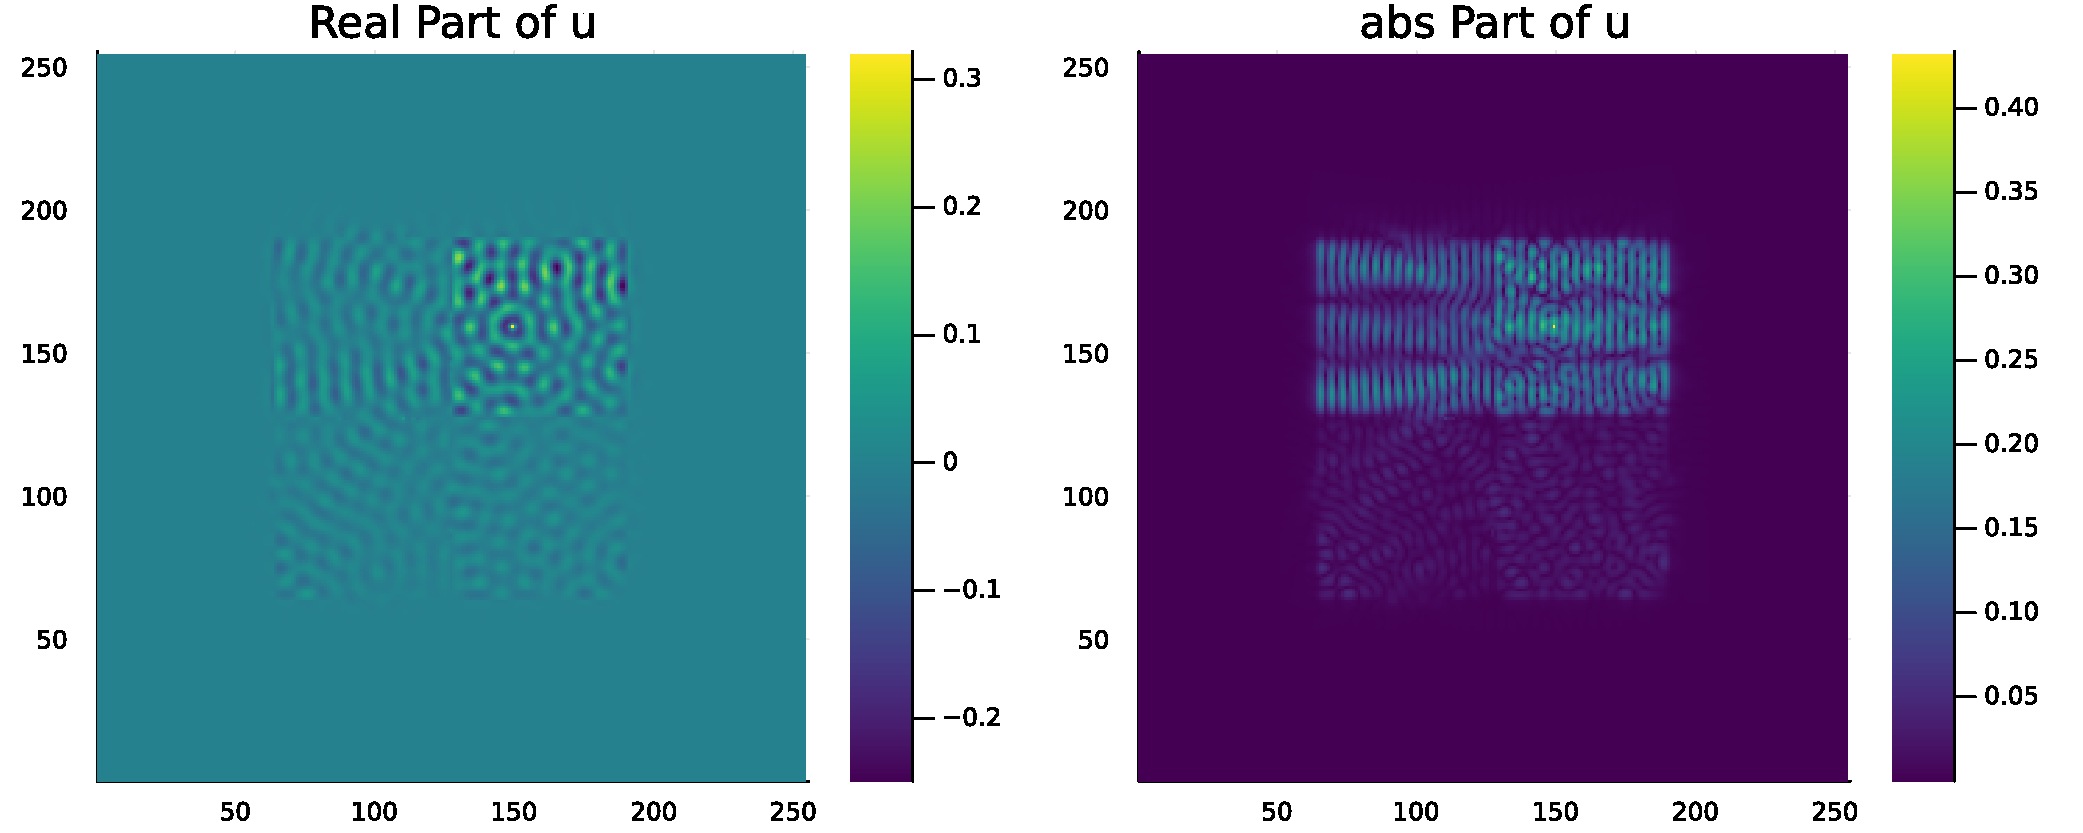
\includegraphics[width=0.8\textwidth]{../plots/gmres_wifi_solution.pdf}
    \caption{Computed Solution for the Wi-Fi Problem}
    \label{fig:gmres_wifi_solution}
\end{figure}


\end{document}
